\documentclass{article}

\usepackage{fullpage}
\usepackage{parskip}
\usepackage{setspace}
\usepackage{mathtools}
\usepackage{tikz}
\usetikzlibrary{arrows}
\usetikzlibrary{decorations.markings}
\usetikzlibrary{calc}
\usepackage{standalone}
\usepackage{float}
\usepackage{caption}
\usepackage{subcaption}
\usepackage{amsmath}
\usepackage{amsfonts}
\usepackage{amsthm}
\usepackage[ruled]{algorithm2e}
\usepackage{adjustbox}
\usepackage{enumerate}
\usepackage{hyperref}
\usepackage[nocompress]{cite}
\usepackage{booktabs}
\usepackage{authblk}

\newtheorem{definition}{Definition}
\newtheorem{theorem}{Theorem}
\newtheorem{proposition}{Proposition}
\newtheorem{lemma}{Lemma}
\newtheorem{remark}{Remark}

\title{Modelling Deadlock in Open Restricted Queueing Networks}
\author{Geraint I. Palmer}
\author{Paul R. Harper\thanks{Corresponding author Prof. Paul Harper, harper@cardiff.ac.uk}}
\author{Vincent A. Knight}
\affil{\small{\textit{School of Mathematics, Cardiff University, Senghennydd Road, Cardiff, CF24 4AG}}}
\date{\today}

\numberwithin{equation}{section}

\begin{document}

\onehalfspacing

\maketitle

\begin{abstract}
Open restricted queueing networks give rise to the phenomenon of deadlock,
whereby some customers may be unable to ever leave a server due to mutual
blocking.
This paper explores deadlock in queueing networks with limited queueing
capacity, presents a method of detecting deadlock in discrete event
simulations, and builds Markov chain models of these deadlocking networks.
The three networks for which Markov models are given include single and
multi-server networks for one and two node systems.
The expected times to deadlock of these models are compared to results obtained
using a simulation of the stochastic process, together with the developed
deadlock detection method.
This paper aims to be of value to simulation modellers of queues.

\textit{Keywords:} queueing, queueing networks, deadlock, Markov models
\end{abstract}

\section{Introduction}

The study and modelling of queueing networks with blocking is an important
tool in many aspects of operational research, both analytically and through
simulation.
These models have applications in many varied settings such as healthcare,
supply chains, manufacturing and communications systems.
However, these types of models have their limitations, due to their potential
to become permanently blocked in deadlock, or a deadly embrace of resources.
These deadlocks can be real and observed in reality, in which case accurate
modelling of deadlock is needed; or they can be a symptom of a model unable to
capture certain behaviours.
This may occur in models where deadlock situations are easily adjusted in
reality.
In this case, such as by swapping two customers, a good understanding of
deadlock is needed in order to model the adjusted reality.

Queueing networks are described as open if customers can enter and leave the
system from the exterior.
Restricted networks are those where at least one service centre has limited
queueing space or capacity before it.
Deadlock is caused by blocking.
This paper considers Type I blocking: after service a customer will be blocked
from joining a queue at another node if that node's queueing capacity is full.
While blocked, that customer remains with its server until space becomes
available at its destination.
During this time that server is unavailable to begin another customer's
service.

For the purposes of this paper, deadlock is defined as follows.\\

\begin{definition}\label{def:deadlock}
    When there is a subset of blocked customers who are blocked directly or
    indirectly by customers in that subset only, then the system is said
    to be in deadlock.
\end{definition}

This implies that a system is in deadlock when at least one service station
permanently ceases to begin or finish any more services, due to circular
blocking.
Figure~\ref{fig:1st_example} shows an open two node restricted queueing
network in deadlock.
The customer at the top server is blocked from entering the bottom node as
there is a full queue, and similarly the customer at the bottom server is
blocked from entering the top node as there is a full queue.
It is clear that by following the rules of blocking defined above, no more
natural movement can happen.
This system is in deadlock as there is a subset of blocked customers (the
customer with server $A_1$ and the customer with server $B_1$) who are only
being blocked by each other.

\begin{figure}[!htbp]
  \begin{center}
  \includestandalone[width=0.4\textwidth]{images/2nodesindeadlock}
  \end{center}
  \caption{Example of an open two node restricted queueing network in deadlock.}
  \label{fig:1st_example}
\end{figure}

This paper is concerned with open restricted queueing networks that experience
Type I blocking.
Exponential service times and Poisson arrivals are assumed.
First in first out, or FIFO service discipline is also assumed.
Throughout the paper service centres will be referred to as nodes, and for the
$i$th node of a queueing network the following notation is used:

\begin{itemize}
  \item $\Lambda_i$ denotes the external arrival rate.
  \item $\mu_i$ denotes the service rate.
  \item $c_i$ denotes the number of parallel servers.
  \item $n_i$ denotes the queueing capacity.
  \item $r_{ij}$ denotes the routing probability from node $i$ to node $j$
  upon completion of service at node $i$.
\end{itemize}

The main contribution of this work to the literature is a formal, rigourous, and
analytical study of deadlock in queueing processes, which has never been done
before.
Methodologies for the detection of deadlock as well as Markovian models of
deadlock are presented.
In particular, this paper looks at detecting when deadlock occurs, and the time
until a deadlock occurs from an empty system.
First, a method for detecting deadlock in simulations of queueing networks is
presented.
Then, Markov models of simple deadlocking queueing networks are built.
This not only contributes a novel theoretic advancement of the study of queueing
networks, but also has the potential for impact in real world queueing networks,
as discussed in Section~\ref{sec:motivatingexample}.

The remainder of this paper is structured as follows:
Section~\ref{sec:motivatingexample} gives a motivating example to put the work
in context.
Section~\ref{sec:litreview} gives an overview of existing literature on the
subject.
Section~\ref{sec:detectingdeadlock} presents a method of detecting deadlock in
simulations of queueing networks.
Section~\ref{sec:markovmodels} presents Markov models of three deadlocking
queueing networks, finds their expected time to deadlock, and compares these
with results obtained through simulation models.


\section{A Motivating Example}\label{sec:motivatingexample}

Here we present a motivating example of a healthcare system.
In this example deadlock may be easily resolved in reality, however analytical
stochastic models and simulations may be restricted by deadlock.
Therefore an understanding of this phenomenon, and an ability to overcome
this effect in discrete event simulations, is essential for modelling this
system.

Consider the interface between secondary care services at a hospital and
community care services.
Patients can be admitted to hospital via a variety of routes (e.g. through
emergency services, or outpatients), and via referral from community care
services.
Patients can begin receiving community care packages after referral from GP,
or via referral from the hospital.
Considering only the hospital and community care services as nodes, this
system is shown in Figure~\ref{fig:motivatingexample}.

\begin{figure}
\begin{center}
\includestandalone[width=0.5\textwidth]{images/motivatingexample}
\end{center}
\caption{Diagram of patient flows at an interface between secondary care
services at a hospital and community care services.}
\label{fig:motivatingexample}
\end{figure}

If there are no free hospital beds, then patients being referred from
community care services will be sustained by community care workers until beds
become available.
If there are no community care packages available, then patients requiring
packages but unfit to return home after a hospital stay will remain in
hospital, blocking beds until a community care package becomes available.
Type I blocking occurs here, as patients and staff do not know the future
capacity of their next destination prior to service.
This type of bed blocking is well known \cite{manzano10}.
This causes problems for patients as they are being cared for in an
inappropriate setting for their condition, and also for the health care
providers as secondary care may be more expensive than primary care, and
resolution of this causes administrative stress.

In this model there is a non-zero probability of everyone at the hospital
blocking beds waiting for community care packages, and everyone at community
care being sustained waiting for beds at the hospital.
Thus the model will exhibit deadlock.
In reality, there is communication between these services and patients can
swap places.
This ensures no deadlock.

Restricted feedback loops that exhibit mutual blocking such as this one have
been observed in real healthcare systems, as described in a case study in
\cite{osoriobierlaire09}.
However the authors here state that this type of blocking ``may be irrelevant
in practice given that the swapping of patients can be identified and carried
out easily''.
In \cite{koizumietal05} a health and community care system is described as
having restricted feedback loops.
However due to ease of modelling, and to avoid the restrictions caused by
deadlock, these feedback loops are omitted from the model.
This emphasises the discrepancies that occur between common modelling
techniques and reality in systems that may reach deadlock.

An understanding of how deadlock behaves in these models will aid the modelling
process.
A deadlock detection method for the simulation model will be invaluable in
modelling realistic deadlock resolution methods, thus ensuring correct models
can be built of systems like this with circular blocking.


\section{Literature Review}\label{sec:litreview}

Restricted queueing networks that exhibit blocking are well discussed in the
literature, both exact \cite{hunt56, baber08, aviitzhakyadin65, koizumietal05,
latoucheneuts80, perrosetal88, gordonnewell67} and approximate methods
\cite{takahashi80, korporaaletal00, onvural90, perrosetal88, dalleryfrein93,
allonetal13, osoriobierlaire09}.
Discussions on restricted queueing networks with feedback loops, that may
exhibit deadlock, are sparse however.
In fact the problem of deadlock in queueing networks has either been ignored,
not studied, or assumed resolved in much of the literature \cite{onvural90,
perrosetal88, osoriobierlaire09}.

Central to the study of deadlock in queueing networks is the concept of
blocking.
In \cite{onvuralperros86} three types of blocking are described.
Type I blocking occurs when a customer is blocked after completing service, and
remains with the server until capacity at their destination node becomes
available.
Type II blocking occurs when a customer declares their destination before
beginning service, and is only granted service if there is available capacity at
their destination node.
In Type III blocking, instead of getting blocked, a customer is required to
repeat their service if there is no capacity at their destination.
This type of blocking comes in two forms, fixed destination where the
customer's destination does not change at each repetition of service, and
random destination, where the customer's destination is re-sampled from a
probability distribution after each repetition.

There has been a body of research around deadlock which doesn't consider the
underlying stochastic structure of the system \cite{coffmanelphick71,
reveliotis15a, reveliotis15b}.
This type of deadlock, also referred to as deadly embraces
\cite{coffmanelphick71}, can potentially occur under the following conditions:

\begin{itemize}
  \item Mutual exclusion: Tasks have exclusive control over resources.
  \item Wait for: Tasks do not release resources while waiting for other
  resources.
  \item No pre-emption: Resources cannot be removed until they have been used
  to completion.
  \item Circular wait: A circular chain of tasks exists, where each task
  requests a resource from another task in the chain.
\end{itemize}

In open restricted queueing networks the mutual exclusion condition is
satisfied as customers cannot share servers; the wait for condition is
satisfied due to the rules of Type I blocking; the no pre-emption condition is
satisfied in networks that have no or non-pre-emptive priority (this paper only
considers networks with no priority); and the circular wait condition is
satisfied if the queueing network contains a cycle where all nodes have limited
queueing capacity.

Allowing a system to reach deadlock can be problematic in cases where
automated systems cannot continue operations, or where simulations cannot
accurately model reality.
In general there are three strategies for dealing with the problem of deadlock
\cite{kawadkaretal14, elmagarmid86, venkateshsmith05, vis06}:

\begin{itemize}
  \item Avoidance, in which decisions are made as time unfolds to avoid
  reaching deadlock.
  \item Prevention, in which the system is designed such that in cannot
  possibly deadlock.
  \item Detection and recovery.
\end{itemize}

Note that \cite{holt72} lists the three strategies as prevention, detection
and crashing, which is equivalent to having no deadlock strategy.
Allowing the system to crash now and again may be more economical in some
systems where deadlocks do not occur often enough to justify the investment
and effort of implementing an avoidance/resolution strategy.

Prevention and avoidance strategies have been used extensively in an area known
as Discrete Event Systems \cite{reveliotis15a, reveliotis15b}.
A number techniques and methods have been used to implement deadlock avoidance
\cite{dijkstra82, kawadkaretal14, viswanadhametal90, ezpeletaetal02,
marchettimunierkordon09, belik90, vis06}.
These techniques generally determine when resources cannot be allocated as
that allocation would lead to deadlock.
In \cite{florianetal08} a priority based deadlock avoidance algorithm is
implemented in a traffic simulation model.
The purpose of the avoidance scheme here is not to reflect deadlock avoidance
in reality, but to avoid deadlocks that will occur in the simulation due to
missing information or incomplete models.

The literature has discussed deadlock prevention in closed queueing networks
under Type I blocking \cite{kunduakyildiz89, liebeherrakyildiz95, onvural90,
schmidtjackman00}.
These have involved determining the minimum queueing space assignment that
prevents deadlock for a given population size, or turning customers away if
certain nodes are full.
For simulation modelling however, prevention and avoidance techniques may not
be appropriate as they can potentially inhibit realism in the simulation by
taking actions that do not occur in the system being modelled
\cite{venkateshetal98}.

A popular method of detecting general deadlock is the use of wait-for graphs,
state-graphs and other variants \cite{cheng90, elmagarmid86, coffmanelphick71,
choetal95, deuermeyeretal97, venkateshetal98, venkateshsmith03,
venkateshsmith05, holt72}.
These wait-for graphs, keep track of all circular wait relations between tasks.
In \cite{coffmanelphick71} dynamic state-graphs are defined with resources as
vertices and requests as edges.
For scenarios where there is only one type of each resource, deadlock arises
if and only if the state-graph contains a cycle.
In \cite{choetal95} `simple bounded circuits' are defined by giving the
vertices and edges of the state graph labels in relation to a reference node.
The existence of these circuits within the state graph indicates if the system
is in deadlock.
A strategy of this type is developed in this paper to detect deadlock in
general queueing systems.

Bipartite entity-resource graphs are used in \cite{holt72, deuermeyeretal97,
venkateshsmith03} to detect deadlock in systems with
both consumable and reusable resources.
Two different types of deadlock are detected, transient deadlock and permanent
deadlock.
A deadlock resolution procedure is proposed that attempts to break cycles in the
entity-resource graph.
This work is furthered in \cite{venkateshetal98} where deadlock is detected
and resolved for situations where entities may request more than one resource.

Deadlock detection and recovery in closed queueing networks through swapping
customers is assumed in \cite{perrosetal88}, with zero transition time assumed
between deadlocked states and the corresponding resolved state.
Time to resolve deadlock may not be negligible in reality.
Deadlock detection and recovery is listed as one of the two possible solutions
for handling deadlock in queueing networks in \cite{akyildiz89}, although
there is no further discussion.

Note that a number of deadlock types are defined in \cite{venkateshetal98}.
The terminology of that paper differs greatly to that used here.
Notably the concept described by their term `Transient deadlock' is not
considered a deadlock situation at all in this paper according to
Definition~\ref{def:deadlock}.





\section{Deadlock Detection}\label{sec:detectingdeadlock}

In order to detect when deadlock has occurred in a queueing network
simulation, a state digraph is used, a form of wait-for graph.
In previous literature on wait-for graphs these are bespoke graphs that
represent system states, where edges denote some form of waiting or blockage
relationships.
Here we present a generic state digraph that is defined for all FIFO
queueing networks that exhibit Type I blocking:\\


\begin{definition}\label{def:statedigraph}
The state digraph $D(t)$ of a queueing network is defined by that network's
state at any time $t$.
Vertices of the state digraph correspond to servers of the network.
A directed edge denotes a blockage relationship in the following manner: if a
customer at the $k$th server of node $i$ is blocked from entering node $j$,
then there are directed edges from the vertex corresponding to node $i$'s
$k$th server to every vertex corresponding to the servers of node $j$.
\end{definition}

To illustrate this concept Figure~\ref{fig:exampledigraphs} shows examples of
queueing networks in and out of deadlock, and the corresponding state digraph
in each case.

\begin{figure}[!htbp]
\begin{center}
  \begin{subfigure}{0.45\textwidth}
    \begin{center}
      \includestandalone[width=0.8\textwidth]{images/exampledigraph_1}
    \end{center}
    \caption{A three node queueing network in deadlock, with state digraph.}
    \label{fig:exampledigraph_deadlock}
  \end{subfigure}
  \hspace{6 mm}
  \begin{subfigure}{0.45\textwidth}
    \begin{center}
      \includestandalone[width=0.8\textwidth]{images/exampledigraph_2}
    \end{center}
    \caption{A three node queueing network not in deadlock, with state
    digraph.}
    \label{fig:exampledigraph_nodeadlock}
    \vspace{6 mm}
  \end{subfigure}
  \begin{subfigure}{0.45\textwidth}
    \begin{center}
      \includestandalone[width=0.8\textwidth]{images/exampledigraph_3}
    \end{center}
    \caption{A two node queueing network in deadlock, with state digraph.}
    \label{fig:exampledigraph2_deadlock}
  \end{subfigure}
  \hspace{6 mm}
  \begin{subfigure}{0.45\textwidth}
    \begin{center}
      \includestandalone[width=0.8\textwidth]{images/exampledigraph_4}
    \end{center}
    \caption{A two node queueing network not in deadlock, with state digraph.}
    \label{fig:exampledigraph2_nodeadlock}
    \vspace{6 mm}
  \end{subfigure}
  \end{center}
  \caption{Examples of state digraphs with their corresponding queueing
  networks.}
  \label{fig:exampledigraphs}
\end{figure}

These graph theoretic terms will be used throughout this paper
\cite{gibbons85, wilson70, bangjensenngutin08}:

\begin{itemize}
  \item Two vertices $v_1$ and $v_2$ are said to be \textit{weakly connected}
  if there is a directed path from $v_1$ to $v_2$ or a directed path from $v_2$
  to $v_1$.
  \item Two vertices $v_1$ and $v_2$ are said to be \textit{strongly
  connected} if there is a directed path from $v_1$ to $v_2$ and a directed
  path from $v_2$ to $v_1$. Note that strongly connected vertices are also
  weakly connected.
  \item A \textit{weakly connected component} of a digraph is a subgraph
  induced by a maximal subset of weakly connected vertices.
  \item A \textit{strongly connected component} of a digraph is a subgraph
  induced by a maximal subset of strongly connected vertices.
  \item The \textit{out-degree} of $v_1$ is the number of out-edges incident to
  $v_1$.
  \item A \textit{sink} is a vertex whose out-degree is zero.
  \item A \textit{knot}, or terminal strong component, is a strongly connected
  component containing no vertices with a path to any vertices outside that
  component.
\end{itemize}

Consider a vertex $v$ in $D(t)$.
Some observations:

\begin{itemize}
  \item If the server corresponding to $v$ is unoccupied, then $v$ has no
  incident edges.
  \item It can be interpreted that all vertices with a path to $v$ correspond to
  servers whose individuals are being blocked directly or indirectly by the
  customer at the server corresponding to $v$.
  \item Similarly it can be interpreted that all vertices that $v$ has a path to
  correspond to servers whose occupants are directly or indirectly blocking
  the customer at the server corresponding to $v$.
  \item It is clear that if all vertices that $v$ has a path to correspond to
  servers occupied by blocked individuals, then the system is deadlocked at time
  $t$.
\end{itemize}

The following results are used detect deadlock for open restricted queueing
networks.

\begin{theorem}\label{thrm:knot}
A deadlocked state arises at time $t$ if and only if $D(t)$ contains a knot.
\end{theorem}

\begin{proof}{Proof}
Consider a queueing network with set of servers $S$.
Consider the state digraph $D(t) = \left(V, E(t)\right)$.
Note that there is a 1-1 pairing between the elements of $S$ and the elements of
$V$, by Definition~\ref{def:statedigraph} of $D(t)$.

\begin{itemize}
  \item Assume the system is in deadlock at time $t$.
By Definition~\ref{def:deadlock} (of deadlock) there exists
$\mathcal{S} \subseteq S$ a subset of servers with blocked customers blocked
only by customers at servers in $\mathcal{S}$.
Consider $\mathcal{V} \subseteq V$ corresponding to $\mathcal{S}$.

For each $s \in \mathcal{S}$ the corresponding $v \in \mathcal{V}$ has at least
one out-edge in $E(t)$ because the customer at $s$ is blocked (by
Definition~\ref{def:statedigraph}).

By Definition~\ref{def:deadlock} every $v \in \mathcal{V}$ has at least one path
in $E(t)$ to a vertex in $\mathcal{V}$, and has no path in $E(t)$ to any vertex
outside of $\mathcal{V}$.

By definition of a knot, there exists
$G = \left(\mathcal{V}, \mathcal{E}\right)$, where $\mathcal{E} \subseteq E(t)$,
such that $G$ is either a knot or a collection of knots.

 \item Assume that $D(t)$ contains a knot
$G = \left(\mathcal{V}, \mathcal{E}\right)$.
Consider $\mathcal{S} \subseteq S$ corresponding to $\mathcal{V}$.

As $G$ is a knot, every $v \in \mathcal{V}$ has an out-edge, thus every customer
at $s \in \mathcal{S}$ is blocked (by Definition~\ref{def:statedigraph}).

As $G$ is a knot, there is no path in $E(t)$ from any $v \in \mathcal{V}$ to any
vertex outside of $\mathcal{V}$.
Therefore every customer at $s \in \mathcal{S}$ is blocked directly or
indirectly by customers at servers in $\mathcal{S}$.

By Definition~\ref{def:deadlock} this implies the system is in deadlock at time
$t$.

\end{itemize}
\end{proof}

The knot condition can be simplified for specific cases.
Theorem~\ref{thrm:wcc_nosink} may offer computational advantages in cases where
it is easier to identify weakly connected components to knots.

\begin{theorem}\label{thrm:wcc_nosink}
For queueing networks:
\begin{enumerate}
  \item with one node
  \item with two nodes, each with two or fewer parallel servers
  \item with a finite amount of nodes, each with a single-server
\end{enumerate}
a deadlocked state arises at time $t$ if and only if $D(t)$ contains a weakly
connected component without a sink.
\end{theorem}

\begin{proof}{Proof}
  To prove the result in one direction, each case is considered separately:
  \begin{enumerate}
  \item
  Consider a one node queueing network.

  If there is deadlock, then all servers are occupied by blocked individuals,
  and so all vertices corresponding to those servers have an out-edge.
  Thus there are no sinks.

  \item
  Consider a two node queueing network, each node with 2 or fewer parallel
  servers.

  If both nodes are involved in the deadlock, so there is at least one
  customer in node 1 blocked from entering node 2, and at least one customer
  from node 2 blocked from entering node 1, then all servers in node 1 and
  node 2 in $D(t)$ will have out edges as they are occupied by a blocked
  individual.
  The servers of node 1 and 2 consist of the entirety of $D(t)$, and so there
  is no sink nodes.

  Now consider the case when only one node is involved in the deadlock.
  Without loss of generality, consider that node 1 is in deadlock with itself,
  then the servers of node 1 have out-edges.
  For the servers of node 2 to be part of that weakly connected component,
  there either needs to be an edge from a server in node 1 to a server in node
  2, or an edge from a server in node 2 to a server in node 1.
  An edge from a server in node 1 to a server in node 2 implies that a
  customer from node 1 is blocked from entering node 2, and so node 1 is not
  in deadlock with itself.
  An edge from a server in node 2 to a server in node 1 implies that a
  customer in node 2 is blocked from entering node 1.
  In this case one server in node 2 has an out-edge.
  Now either the other server of node two is empty or still in service, and so
  isn't part of that weakly connected component, or the other server's
  customer is blocked and so has an out edge.
  Thus there are no sinks.

  \item
  Consider a queueing network with $N$ nodes, each with a single-server.

  If $1 \leq n \leq N$ nodes are involved in the deadlock, then each server in
  those $n$ nodes has a blocked customer, and so the corresponding vertex in the
  state digraph has an out-edge.

  Of the nodes not involved in that deadlock, the vertices corresponding to
  their servers can only be in the same weakly connected component if:

  \begin{itemize}
    \item They contain a blocked individual that is blocked to the nodes
    involved in the deadlock.
    \item Individuals in the deadlocked nodes are blocked to them.
  \end{itemize}

  In the first case, the vertices corresponding to the servers in those nodes
  will all have an out-edge.
  In the second case it is implied that the customers at servers in deadlocked
  nodes are blocked to both a node in deadlock, and a node not in deadlock.
  Which is not possible (customers can only be blocked to one location at a
  time).

  Thus there are no sinks.
  \end{enumerate}

To prove the result in the other direction, is equivalent to proving that a
weakly connected component without a sink contains a knot:

\begin{itemize}
  \item Consider a weakly connected component, $G$, of $D(t)$.
  \item Assume $G$ contains no knots. By definition of a knot, this implies:
  \begin{itemize}
    \item $G$ contains a sink; or
    \item $G$ contains a vertex with a path to another vertex outside of $G$
    (contradicting the fact that $G$ is a weakly connected component).
  \end{itemize}
\end{itemize}

Thus the existence of a weakly connected component without a sink in $D(t)$
implies that there is a knot in $D(t)$, and the result follows by applying
Theorem~\ref{thrm:knot}.
\end{proof}

In the general case using the result of Theorem~\ref{thrm:wcc_nosink} is not
sufficient to detect deadlock.
In order to illustrate this, consider the following counter-example of a two
node queueing network, where node $A$ has two servers, node $B$ has three
servers.
Begining with all servers occupied by customers in service and full queues.
The customer at server $A_1$ is blocked to node $A$.
The customer at server $B_1$ is blocked to node $A$.
The customer at server $B_2$ is blocked to node $B$.
The customer at server $A_2$ is blocked to node $A$.
Node $A$ is a deadlocked.
The resulting state digraph, shown in Figure~\ref{fig:counter_example}, has a
weakly connected component with a sink.

\begin{figure}
\begin{center}
\includestandalone[width=0.4\textwidth]{images/counter_example_digraph_1}
\end{center}
\caption{State digraph of the counter-example.}
\label{fig:counter_example}
\end{figure}

For the purposes of this paper, a simulation model is used to verify that the
results of this section and the analytical model in
Section~\ref{sec:markovmodels} are in agreement.
Specifically the time taken to reach deadlock from an empty system is
investigated, and the simulation model gives information on the distribution
of times to deadlock.
The model is built using Ciw \cite{ciwpython}.
This is an object oriented framework in Python \cite{python15}, with care
taken to ensure reproducibility of the results \cite{hongetal15}.

The digraph \(D(t)\) is implemented as an attribute of the queueing network
and is updated at the appropriate events.
Note that a brute force algorithm is used to check whether any strongly
connected component of $D(t)$ is a knot in order to implement
Theorem~\ref{thrm:knot}.
More efficient algorithms could be used for other specific use cases.

In the next section Markov models of three queueing networks are built, and
their deadlock properties discussed.


\section{Markovian Models of Deadlocking Queueing Networks}\label{sec:markovmodels}

The following three networks describe all possible configurations of
deadlocking queueing networks with two or fewer nodes:

\begin{enumerate}
  \item Open one node, multi-server restricted queueing network with feedback
  loop. (Section~\ref{sec:1nodeMS}) \label{itm:1Nms}
  \item Open two node, multi-server restricted queueing network with routes
  between nodes. (Section~\ref{sec:2nodeMS}) \label{itm:2Nmss}
  \item Open two node, multi-server restricted queueing network with routes
  between nodes and self-loops. \label{itm:2Nmsf}
\end{enumerate}

In this section Markov models are built for networks~\ref{itm:1Nms} and
\ref{itm:2Nmss}, and their expected time to deadlock found.
The state space for network~\ref{itm:2Nmsf} is too large to model in a similar
way to the others, and so isn't considered in this paper.
A single server version is modelled however (Section~\ref{sec:2nodeselfloops}),
and the multi-server system is briefly discussed in
Section~\ref{sec:conclusions}.

In general a continuous Markov chain model of a deadlocking queueing network
is defined by a set of states $S$ and the transition rates between these
states $q_{s_1,s_2}$.
Each state $s \in S$ uniquely defines a configuration of customers around the
queueing network.
Deadlocked states are also present, either denoted by that specific
configuration of customers, or by negative numbers, for example $(-1)$.
Deadlocked states cannot transition to any other state, and so are absorbing
states of the Markov chain.
Therefore any queueing network that can experience deadlock is guaranteed to
experience deadlock, as absorbing Markov chains are guaranteed to enter one of
its absorbing states.

The expected time until deadlock is reached is equivalent to the expected time
to absorption of the Markov chain, which can be found using classic results~\cite{stewart09}.
The continuous Markov chain is converted to a discrete time absorbing Markov
chain with canonical form:

\begin{equation*}
P = \left(\begin{array}{cc} T & U\\ 0 & I \end{array} \right)
\end{equation*}

where $I$ is the identity matrix.
Now the expected number of time steps until absorption starting from the
$i\text{th}$ state is the $i\text{th}$ element of the vector

\begin{equation} \label{eq:abs_probs}
  (I - T)^{-1}e
\end{equation}

where $e$ is a vector of 1s.

Therefore by discretising the continuous Markov chain and ensuring the correct
order of states, the expected number of time steps to absorption, which
corresponds to deadlock, can be found.
This can be converted back to continuous time by multiplying with the time
step used in the discretisation process.

When there is more than one deadlocked state, there is more than one absorbing
state in the Markov chain.
Here the expected time to absorption is the expected time to a deadlocked
state, whichever one that may be.

\subsection{One Node Multi-Server}\label{sec:1nodeMS}


Consider the open one node multi-server restricted queueing network shown in
Figure~\ref{fig:queueingnetwork_1nodemulti}.
This shows an \(M/M/c/n\) queue where customers arrive at a rate of $\Lambda$
and served at a rate $\mu$.
Once a customer has finished service they rejoin the queue with probability
$r_{11}$, and so exit the system with probability $1 - r_{11}$.

\begin{figure}[!htbp]
  \begin{center}
  \includestandalone[width=0.75\textwidth]{images/1nodemultiserver}
  \end{center}
  \caption{An open one node multi-server restricted queueing network.}
  \label{fig:queueingnetwork_1nodemulti}
\end{figure}

The state space is given by:
    \[S = \{i\in\mathbb{N} \nonscript\; | \nonscript\; 0 \leq i \leq n + 2c\}\]
where \(i\) denotes the number of individuals in the system plus the number of
individuals who are blocked.
For example, $i=n+c+2$ denotes a full system, $n+c$ individuals in the node,
and 2 of those individuals are also blocked.
The state $i=n+2c$ denotes the deadlocked state, that is every customer with a
server is blocked.

Define $\delta = i_2 - i_1$ for all $i_k \in S$.
The transitions are given by Equations~\ref{eqn:1msA} and \ref{eqn:1msB}.

\begin{equation}\label{eqn:1msA}
  q_{i_1, i_2} = \left\{
  \begin{array}{rr}
    \left. \begin{array}{rr}
      \Lambda & \text{if } \delta = 1 \\
      (1-r_{11})\mu\text{min}(i, c) & \text{if } \delta = -1 \\
      0 & \text{otherwise}
    \end{array} \right\} & \text{if } i_1 < n + c \\
  \end{array} \right.
\end{equation}

\begin{equation}\label{eqn:1msB}
  q_{i_1, i_2} = \left\{
  \begin{array}{rr}
    \left. \begin{array}{rr}
      (c-b)r_{11}\mu & \text{if } \delta = 1 \\
      (1-r_{11})(b-k)\mu & \text{if } \delta = -b-1\\
      0 & \text{otherwise}
    \end{array} \right\} & \text{if } i_1 = n + c + b \\
  \end{array} \right.
  \quad \forall \quad 0 \leq b \leq c
\end{equation}

where $b$ denotes the number of blocked customers.
The Markov chain is shown in Figure~\ref{fig:1nodeMCms}.

\begin{figure}[!htbp]
    \begin{center}
    \includestandalone[width=\textwidth]{images/MC1nodemultiserv_bw}
    \end{center}
    \caption{Diagrammatic representation of the Markov chain for a
    multi-server one node system.}
    \label{fig:1nodeMCms}
\end{figure}

Figure~\ref{fig:timestodeadlock1nodemultiserver} shows the effect of varying
the parameters of the above Markov model.
Base parameters of $\Lambda = 6$, $n = 3$, $\mu = 2$, $r_{11} = 0.5$ and
$c = 2$ were used.

\begin{figure}[!htbp]
  \begin{center}
  \begin{subfigure}[b]{0.48\textwidth}
    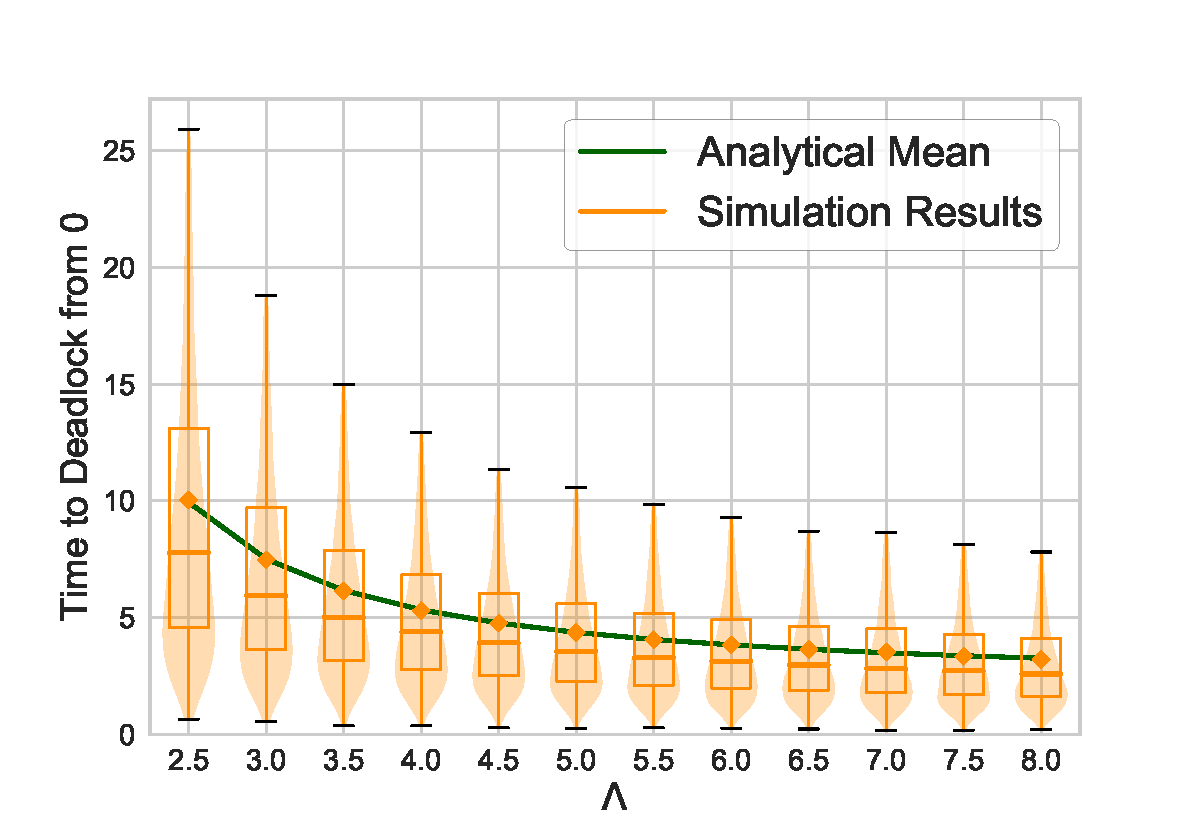
\includegraphics[width=\textwidth]{images/1Nms_varyL}
    \caption{Varying $\Lambda$}
    \label{fig:1Nms_L}
  \end{subfigure}
  \begin{subfigure}[b]{0.48\textwidth}
    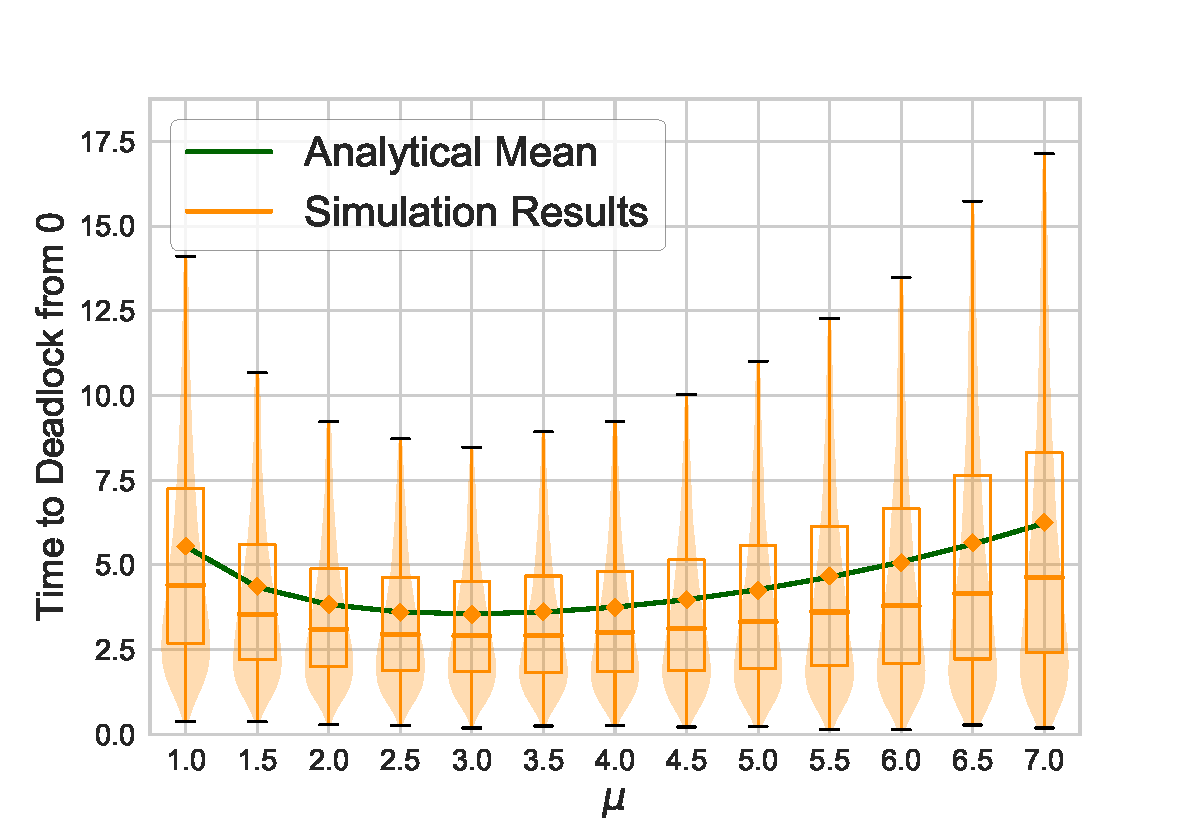
\includegraphics[width=\textwidth]{images/1Nms_varymu}
    \caption{Varying $\mu$}
    \label{fig:1Nms_mu}
  \end{subfigure}\\
  \begin{subfigure}[b]{0.48\textwidth}
    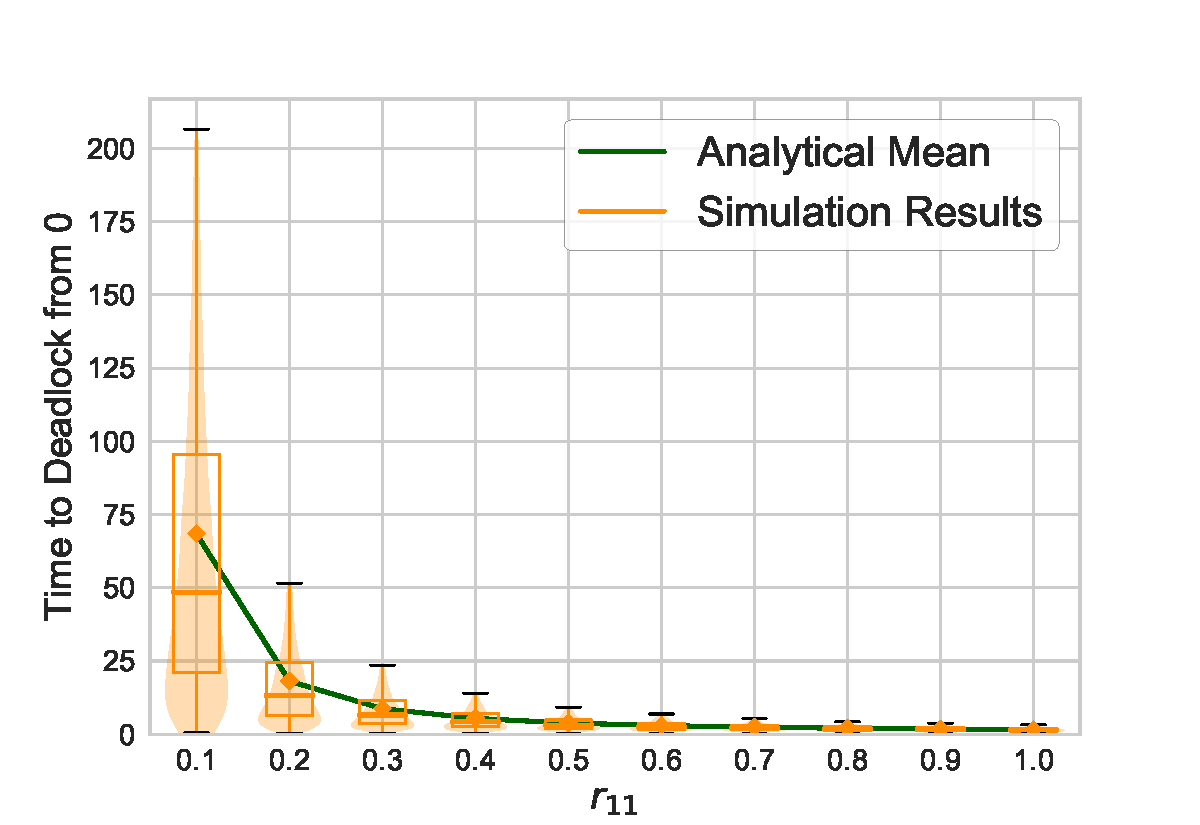
\includegraphics[width=\textwidth]{images/1Nms_varyr11}
    \caption{Varying $r_{11}$}
    \label{fig:1Nms_r11}
  \end{subfigure}
  \begin{subfigure}[b]{0.48\textwidth}
    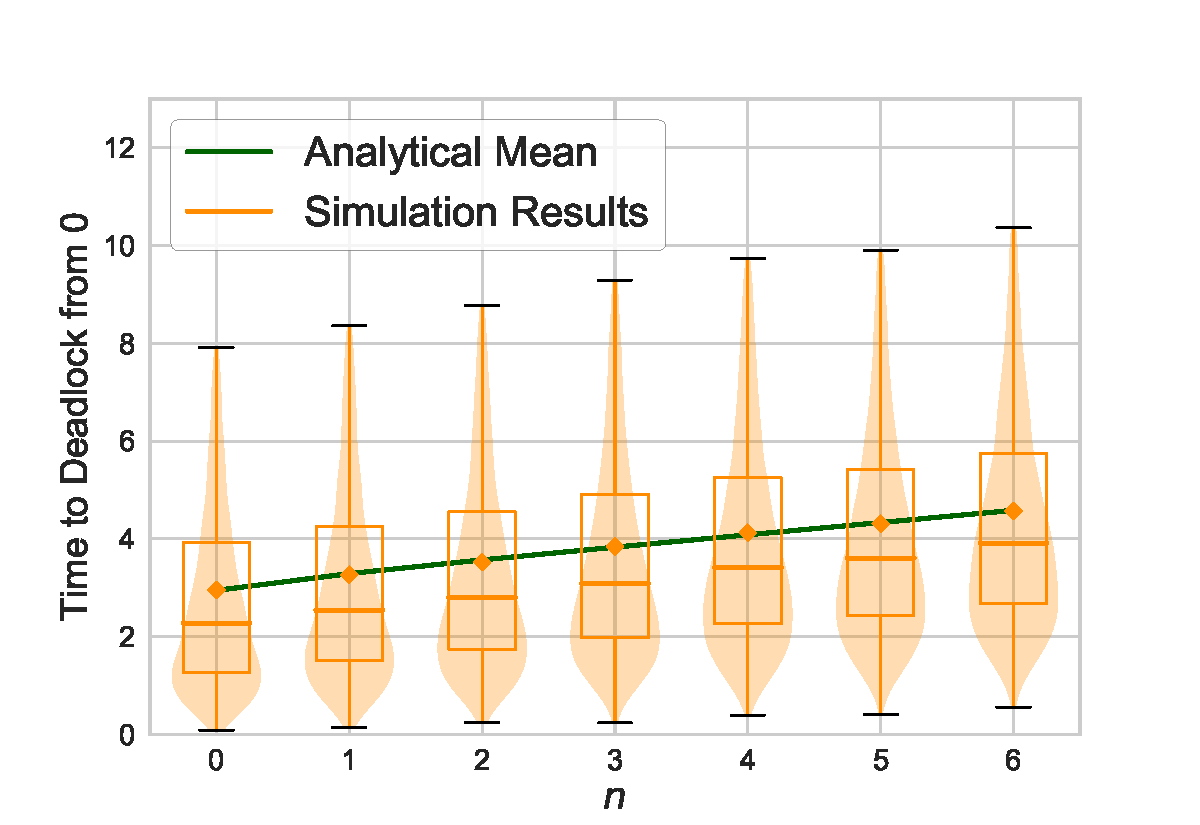
\includegraphics[width=\textwidth]{images/1Nms_varyn}
    \caption{Varying $n$}
    \label{fig:1Nms_n}
  \end{subfigure}\\
  \begin{subfigure}[b]{0.48\textwidth}
    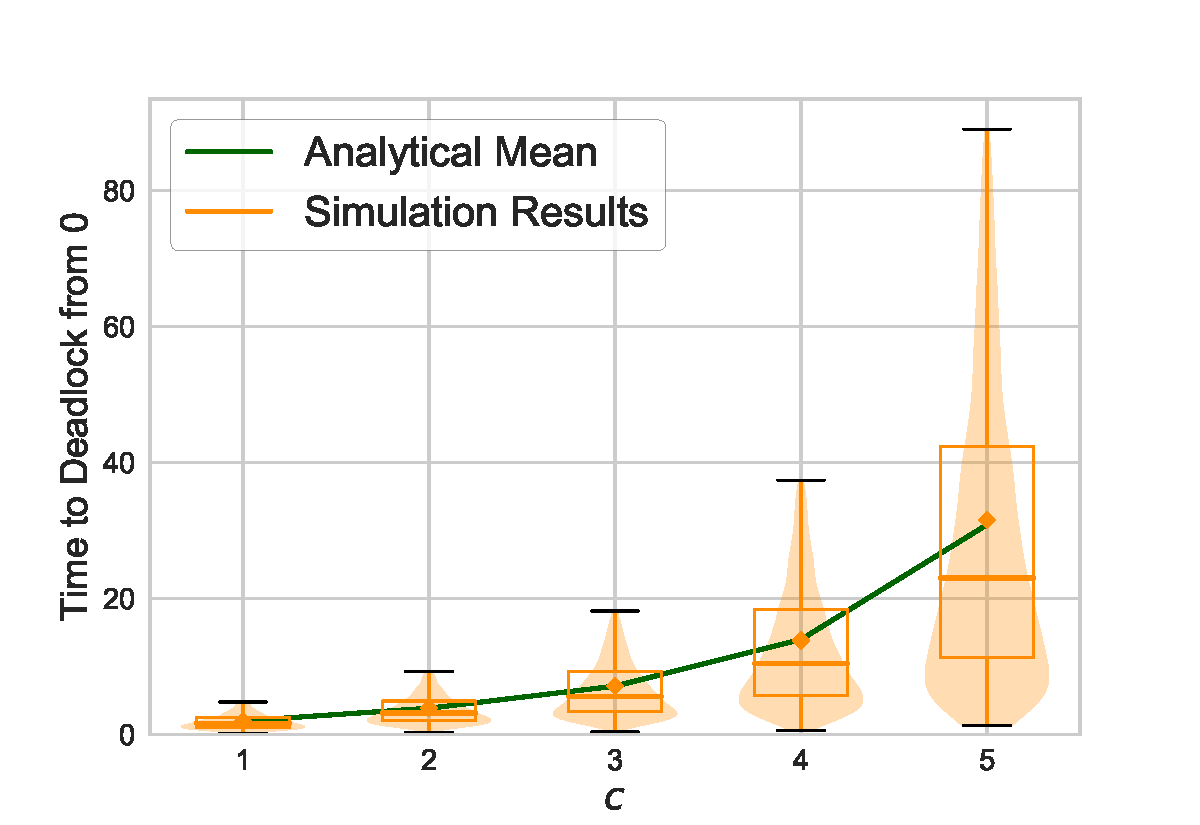
\includegraphics[width=\textwidth]{images/1Nms_varyc}
    \caption{Varying $c$}
    \label{fig:1Nms_c}
  \end{subfigure}
  \end{center}
  \caption{Time to deadlock in multi-server one node system, analytical \&
  simulation results (10,000 repetitions).}
  \label{fig:timestodeadlock1nodemultiserver}
\end{figure}

It can be seen that increasing the arrival rate $\Lambda$ and the routing
probability $r_{11}$ results in reaching deadlock faster.
This is intuitive as increasing these parameters results in the queue filling
up quicker.
Increasing the queueing capacity $n$ results in reaching deadlock later.
Again this is intuitive, as increasing the queueing capacity allows more
customers in the system before becoming deadlocked.

Increasing the amount of servers has a similar effect to increasing the
queueing capacity, there are now more transient states to go through before
reaching the deadlocked state.
Varying the amount of servers has a greater effect on the time to deadlock
however, as any states in which customers are blocked, $i \in [n+c+1, n+2c]$,
can jump back to state $i=n+c-1$ simply with a service where the customer
doesn't rejoin the queue.
Increasing the amount of servers also increases the rate at which customer leave
the system, but not the rate at which customers enter the system.
This means that the rate of increase of the number of customers in the system
increases, however the rate of decrease of number of customers in the system
does not change, thus it would take longer to reach a full system, and thus
deadlock.

The behaviour as the service rate $\mu$ varies is not monotonic, as the
service rate contributes towards both moving customers from the system and
allowing customers to rejoin the queue, causing blockages and deadlock.
If the function $\omega(\mu)$ describes the expected time to deadlock of this
system as the service rate $\mu$ varies, and all other parameters are
fixed, then it is observed that $\omega(\mu)$ has one critical point and is a
local minimum for $\mu \in (0, \infty)$.

The observed bowl shaped curve can be explained by considering the effect of
varying the service rate.
At $\lim_{\mu \to 0} \omega(\mu)$ there is infinite service time, and so
infinite time until deadlock.
At $\lim_{\mu \to \infty} \omega(\mu)$ there is zero service time, the queue can
never fill up, and so infinite time to deadlock.
At low service rates below a certain threshold $\hat{\mu}$, the arrival rate is
relatively large compared to the service rate, and we can assume a saturated
system.
At this point services in which a customer exits the system do not have much of
an effect on the system state, as we can assume another arrival immediately.
However services in which a customer wishes to rejoin the queue results in a
blockage as the system is saturated.
Therefore, increasing the service rate here increases the chance of a blockage,
and so the chance of deadlock.
Above $\hat{\mu}$ the service rate is large enough that we cannot assume a
saturated system, and so services in which the customer exits the system do have
an affect on the number of customers in the system.
Thus increasing the service rate incrases the rate at which customers are
removed from the system, and so there is less chance of reaching deadlock.


\subsection{Two Node Multi-Server without Self-Loops}\label{sec:2nodeMS}

Consider the open two node multi-server restricted queueing network shown in
Figure~\ref{fig:queueingnetwork_2nodemulti}.
This shows two \(M/M/c_i/n_i\) queues, with service rates $\mu_i$ and external
arrival rates $\Lambda_i$.
All routing probabilities $r_{ij}$ may be positive apart from self-loops
$r_{ii}$, for each node $i$.
Note that this system is equivalent to the one described in
Section~\ref{sec:motivatingexample}.

\begin{figure}[!htbp]
  \begin{center}
  \includestandalone[width=0.75\textwidth]{images/2nodemultiserver}
  \end{center}
  \caption{An open two node multi-server restricted queueing network.}
  \label{fig:queueingnetwork_2nodemulti}
\end{figure}

The state space is given by:
    \[S = \{(i,j)\in\mathbb{N}^2 \nonscript\; | \nonscript\; i \leq n_1+c_1+j, \nonscript\; j \leq n_2+c_2+i\}\]
where $i$ denotes the number of individuals at Node 1 plus the number of
individuals blocked waiting to enter Node 1, and $j$ denotes the number of
individuals at Node 2 plus the number of individuals blocked waiting to enter
Node 2.
For example, $(i, j) = (n_1+c_1+2, n_2+c_2+1)$ denotes a full system,
$n_1+c_1$ individuals at Node 1, two of whom are blocked waiting to enter
Node 2; $n_2+c_2$ individuals at Node 2, one of whom is blocked waiting to
enter Node 1.
The state $(i, j) = (n_1+c_1+c_2, n_2+c_2+c_1)$ denotes the deadlocked state.

The Markov chain is shown in Figure~\ref{fig:2nodeMCms}.

\begin{figure}[!htbp]
    \includestandalone[width=\textwidth]{images/MC2nodemultiserv_bw}
    \caption{Diagrammatic representation of the Markov chain for a
    multi-server two node system without self-loops with $n_1=1$,
    $n_2=c_1=c_2=2$. The deadlocked state is $(5,6)$.}
    \label{fig:2nodeMCms}
\end{figure}

Define $\delta = (i_2, j_2) - (i_1, j_1)$, $b_1 = \max(0, i_1-n_1-c_1)$,
$b_2 = \max(0, i_2-n_2-c_2)$, $s_1 = \min(i_1, c_1)-b_2$ and
$s_2 = \min(i_2, c_2)-b_1$ for all $(i_k, j_k) \in S$.
Then the transitions $q_{(i_1, j_1),(i_2, j_2)}$ are given by
Table~\ref{tab:transitionsmultierv}.


\begin{table}
\begin{center}
\resizebox{\textwidth}{!}{
\begin{tabular}{ l l l l }
  \toprule
  & $j_1 < n_2 + c_2$ & $j_1 = n_2 + c_2$ & $ j_1 > n_2 + c_2$ \\
  \midrule
  $i_1 < n_1 + c_1$ & \begin{tabular}{ l } $\Lambda_1$ if $\delta = (1, 0)$ \\ $\Lambda_2$ if $\delta = (0, 1)$ \\ $r_{12}s_1\mu_1$ if $\delta = (-1, 1)$ \\ $r_{21}s_2\mu_2$ if $\delta = (1, -1)$ \\ $(1-r_{12})s_1\mu_1$ if $\delta = (-1, 0)$ \\ $(1-r_{21})s_2\mu_2$ if $\delta = (0, -1)$ \end{tabular} & \begin{tabular}{ l } $\Lambda_1$ if $\delta = (1, 0)$ \\ $r_{12}s_1\mu_1$ if $\delta = (0, 1)$ \\ $r_{21}s_2\mu_2$ if $\delta = (1, -1)$ \\ $(1-r_{12})s_1\mu_1$ if $\delta = (-1, 0)$ \\ $(1-r_{21})s_2\mu_2$ if $\delta = (0, -1)$ \end{tabular} & \begin{tabular}{ l } $\Lambda_1$ if $\delta = (1, 0)$ \\ $r_{12}s_1\mu_1$ if $\delta = (0, 1)$ \\ $r_{21}s_2\mu_2$ if $\delta = (0, -1)$ \\ $(1-r_{12})s_1\mu_1$ if $\delta = (-1, 0)$ \\ $(1-r_{21})s_2\mu_2$ if $\delta = (-1, -1)$ \end{tabular} \\
  \midrule
  $i_1 = n_1 + c_1$ & \begin{tabular}{ l } $\Lambda_2$ if $\delta = (0, 1)$ \\ $r_{12}s_1\mu_1$ if $\delta = (-1, 1)$ \\ $r_{21}s_2\mu_2$ if $\delta = (1, 0)$ \\ $(1-r_{12})s_1\mu_1$ if $\delta = (-1, 0)$ \\ $(1-r_{21})s_2\mu_2$ if $\delta = (0, -1)$ \end{tabular} & \begin{tabular}{ l } $r_{12}s_1\mu_1$ if $\delta = (0, 1)$ \\ $r_{21}s_2\mu_2$ if $\delta = (1, 0)$ \\ $(1-r_{12})s_1\mu_1$ if $\delta = (-1, 0)$ \\ $(1-r_{21})s_2\mu_2$ if $\delta = (0, -1)$ \end{tabular} & \begin{tabular}{ l } $r_{12}s_1\mu_1$ if $\delta = (0, 1)$ \\ $r_{21}s_2\mu_2$ if $\delta = (1, 0)$ \\ $(1-r_{12})s_1\mu_1$ if $\delta = (-1, 0)$ \\ $(1-r_{21})s_2\mu_2$ if $\delta = (-1, -1)$ \end{tabular} \\
  \midrule
  $i_1 > n_1 + c_1$ & \begin{tabular}{ l } $\Lambda_2$ if $\delta = (0, 1)$ \\ $r_{12}s_1\mu_1$ if $\delta = (-1, 0)$ \\ $r_{21}s_2\mu_2$ if $\delta = (1, 0)$ \\ $(1-r_{12})s_1\mu_1$ if $\delta = (-1, -1)$ \\ $(1-r_{21})s_2\mu_2$ if $\delta = (0, -1)$ \end{tabular} & \begin{tabular}{ l } $r_{12}s_1\mu_1$ if $\delta = (0, 1)$ \\ $r_{21}s_2\mu_2$ if $\delta = (1, 0)$ \\ $(1-r_{12})s_1\mu_1$ if $\delta = (-1, -1)$ \\ $(1-r_{21})s_2\mu_2$ if $\delta = (0, -1)$ \end{tabular} & \begin{tabular}{ l } $r_{12}s_1\mu_1$ if $\delta = (0, 1)$ \\ $r_{21}s_2\mu_2$ if $\delta = (1, 0)$ \\ $(1-r_{12})s_1\mu_1$ if $\delta = (-\min(b_1+1,b_2+1), -\min(b_1,b_2+1))$ \\ $(1-r_{21})s_2\mu_2$ if $\delta = (-\min(b_1+1,b_2), -\min(b_1+1,b_2+1))$ \end{tabular} \\
  \bottomrule
\end{tabular}
}
\caption{Table of transitions $q_{(i_1, j_1),(i_2, j_2)}$ for a multi-server
two node network.}
\label{tab:transitionsmultierv}
\end{center}
\end{table}


The values $b_1$ and $b_2$ correspond to the number of people blocked to
Node 1 and Node 2 respectively.
The values $s_1$ and $s_2$ correspond to the amount of people currently in
service at Node 1 and Node 2 respectively.

Figure~\ref{fig:timestodeadlock2nodemultiserver} shows the effect of varying
the parameters of the above Markov model.
Base parameters of $\Lambda_1 = 9$, $\Lambda_2 = 7.5$, $n_1 = 2$, $n_2 = 1$,
$\mu_1 = 5.5$, $\mu_2 = 6.5$, $r_{12} = 0.7$, $r_{21} = 0.6$, $c_1 = 2$ and
$c_2 = 2$ were used.
Only plots for the parameter corresponding to Node 1 are shown, Node 2 shows
similar behaviour.
Similar behaviour is observed to that seen in
Figure~\ref{fig:timestodeadlock1nodemultiserver}.

\begin{figure}[!htbp]
  \begin{center}
  \begin{subfigure}[b]{0.48\textwidth}
    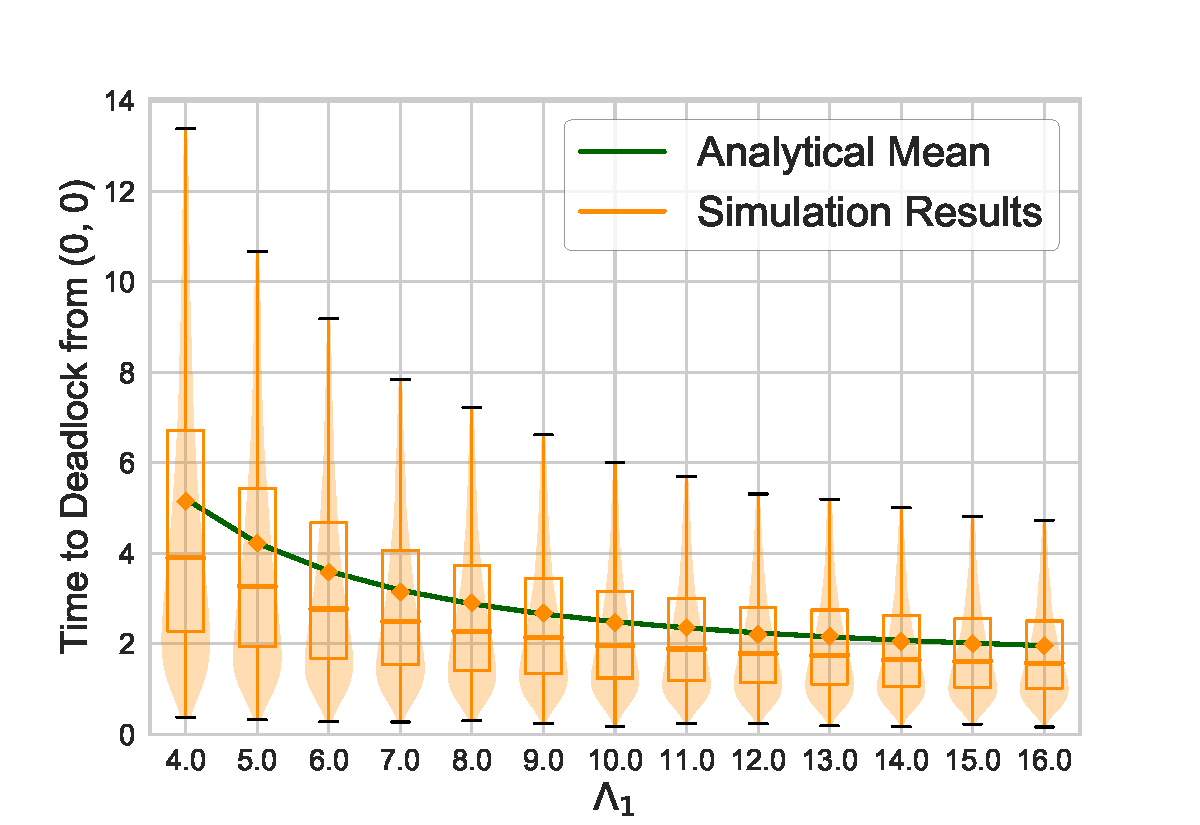
\includegraphics[width=\textwidth]{images/2Nms_varyL1}
    \caption{Varying $\Lambda_1$}
    \label{fig:2Nms_L}
  \end{subfigure}
  \begin{subfigure}[b]{0.48\textwidth}
    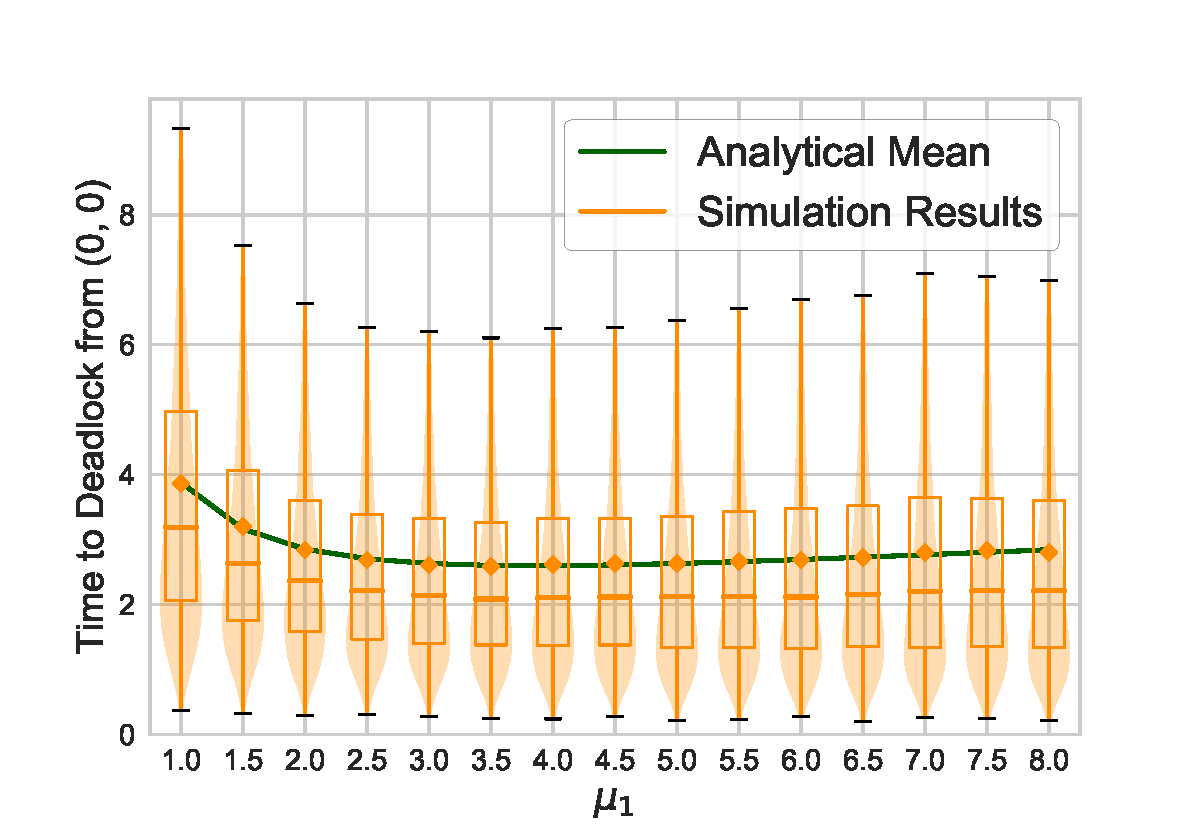
\includegraphics[width=\textwidth]{images/2Nms_varymu1}
    \caption{Varying $\mu_1$}
    \label{fig:2Nms_mu}
  \end{subfigure}\\
  \begin{subfigure}[b]{0.48\textwidth}
    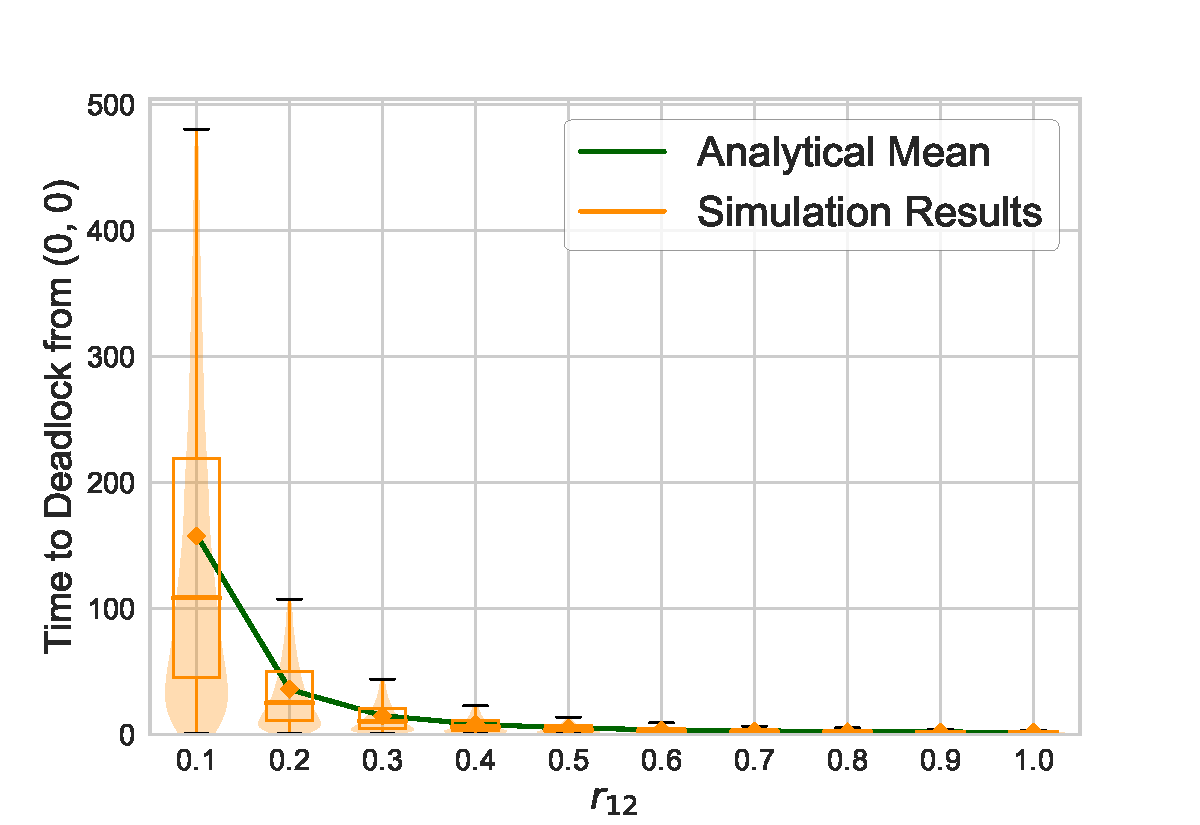
\includegraphics[width=\textwidth]{images/2Nms_varyr12}
    \caption{Varying $r_{12}$}
    \label{fig:2Nms_r11}
  \end{subfigure}
  \begin{subfigure}[b]{0.48\textwidth}
    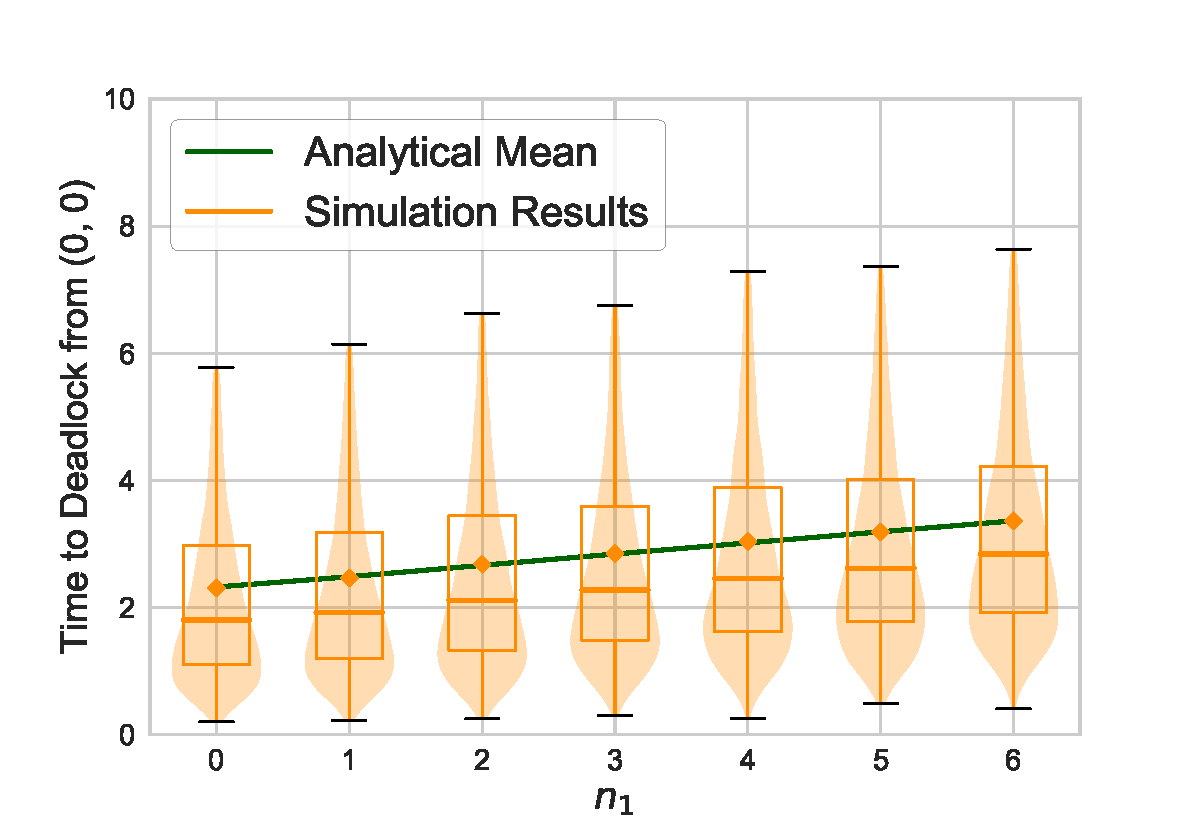
\includegraphics[width=\textwidth]{images/2Nms_varyn1}
    \caption{Varying $n_1$}
    \label{fig:2Nms_n}
  \end{subfigure}\\
  \begin{subfigure}[b]{0.48\textwidth}
    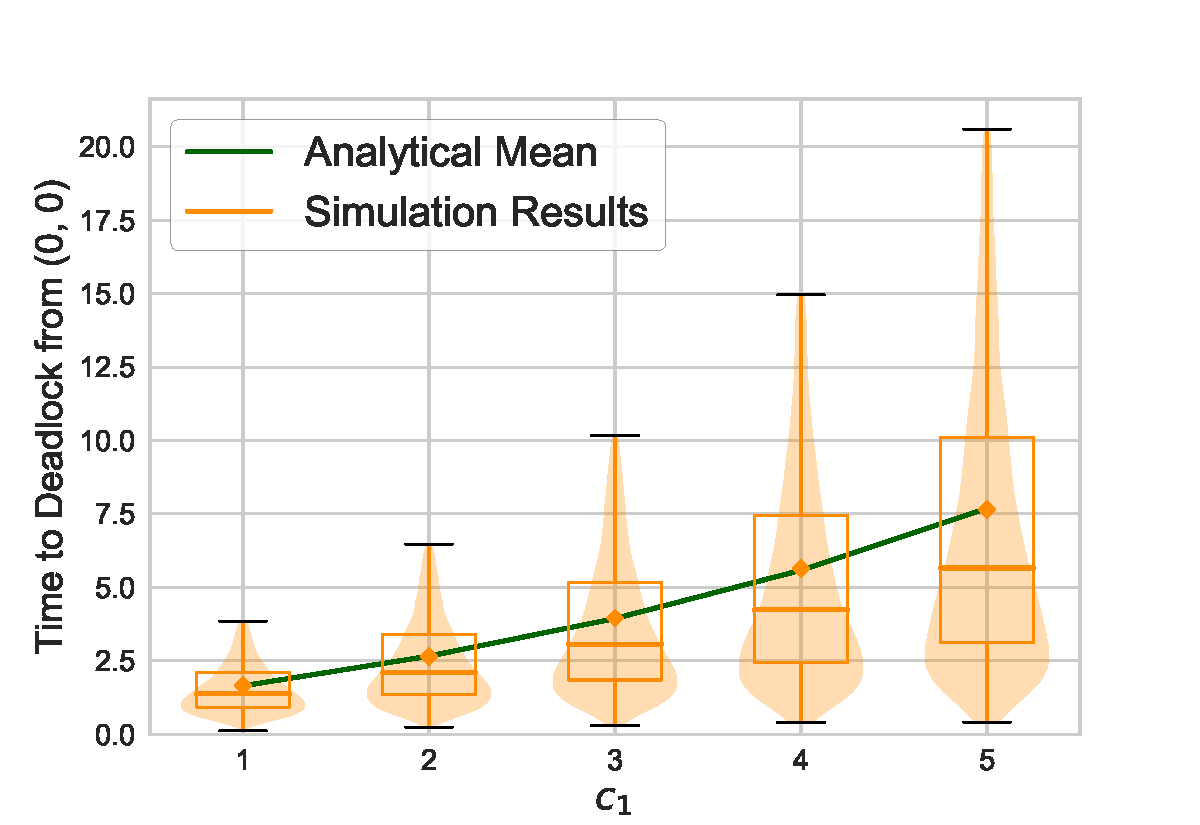
\includegraphics[width=\textwidth]{images/2Nms_varyc1}
    \caption{Varying $c_1$}
    \label{fig:2Nms_c}
  \end{subfigure}
  \end{center}
  \caption{Time to deadlock in multi-server two node system without self loops,
  analytical \& simulation results (10,000 repetitions).}
  \label{fig:timestodeadlock2nodemultiserver}
\end{figure}


\subsection{Two Node Single-Server with Self-Loops}\label{sec:2nodeselfloops}

Consider the open two node single-server restricted queueing network shown in
Figure~\ref{fig:queueingnetwork_2nodesfeedback}.
This shows two \(M/M/1/n_i\) queues with service rates $\mu_i$  and external
arrival rates $\Lambda_i$.
All routes are possible, where the routing probability from node $i$ to node
$j$ is denoted by $r_{ij}$.

\begin{figure}[!htbp]
  \begin{center}
  \includestandalone[width=0.75\textwidth]{images/2nodefeedbackexample}
  \end{center}
  \caption{An open two node single-server restricted queueing network.}
  \label{fig:queueingnetwork_2nodesfeedback}
\end{figure}

The state space is given by:
    \[S = \{(i,j)\in\mathbb{N}^2 \nonscript\; | \nonscript\; 0 \leq i + j \leq n_1 + n_2 + 2 \}\cup\{(-1), (-2), (-3)\}\]

    where \(i\) denotes the number of individuals:
        \begin{itemize}
            \item In service or waiting at the first node.
            \item Occupying a server but having finished service at the
                second node waiting to join the first.
        \end{itemize}
    where \(j\) denotes the number of individuals:
        \begin{itemize}
            \item In service or waiting at the second node.
            \item Occupying a server but having finished service at the
                first node waiting to join the second.
        \end{itemize}
    and the state $(-3)$ denotes the deadlocked state caused by both nodes;
    $(-1)$ denotes the deadlocked state caused by the first node only; and
    $(-2)$ denotes the deadlocked state caused by the second node only.

Define $\delta = (i_2, j_2) - (i_1, j_1)$ for all $(i_k, j_k) \in S$.
The transitions are given by Equations~\ref{eqn:2nssfA}, \ref{equ:todeadlock2},
\ref{equ:todeadlock3} and \ref{eqn:2nssfB}.

\begin{equation}\label{eqn:2nssfA}
  q_{(i_1, j_1),(i_2, j_2)} = \left\{
  \begin{array}{rr}
    \left. \begin{array}{rr}
      \Lambda_1 & \text{if } i_1 < n_1 + 1 \\
      0 & \text{otherwise}
    \end{array} \right\} & \text{if } \delta = (1, 0) \\
    \left. \begin{array}{rr}
      \Lambda_2 & \text{if } j_1 < n_2 + 1 \\
      0 & \text{otherwise}
    \end{array} \right\} & \text{if } \delta = (0, 1) \\
    \left. \begin{array}{rr}
      (1 - r_{11} - r_{12})\mu_1 & \text{if } j_1 < n_2 + 2 \\
      0 & \text{otherwise}
    \end{array} \right\} & \text{if } \delta = (-1, 0) \\
    \left. \begin{array}{rr}
      (1 - r_{21} - r_{22})\mu_2 & \text{if } i_1 < n_1 + 2 \\
      0 & \text{otherwise}
    \end{array} \right\} & \text{if } \delta = (0, -1) \\
    \left. \begin{array}{rr}
      r_{12}\mu_1 & \text{if } j_1 < n_2 + 2 \text{ and } (i_1, j_1) \neq (n_1 + 2, n_2) \\
      0 & \text{otherwise}
    \end{array} \right\} & \text{if } \delta = (-1, 1) \\
    \left. \begin{array}{rr}
      r_{21}\mu_2 & \text{if } i_1 < n_1 + 2 \text{ and } (i_1, j_1) \neq (n_1, n_2 + 2) \\
      0 & \text{otherwise}
    \end{array} \right\} & \text{if } \delta = (1, -1) \\
    0 & \text{otherwise}
  \end{array} \right.
\end{equation}

\begin{equation}\label{equ:todeadlock2}
  q_{(i_1, j_1), (-1)} = \left\{
  \begin{array}{rr}
    r_{11}\mu_1 & \text{if } i > n_1 \text{ and } j < n_2 + 2 \\
    0 & \text{otherwise}
  \end{array}
  \right.
\end{equation}

\begin{equation}\label{equ:todeadlock3}
  q_{(i_1, j_1), (-2)} = \left\{
  \begin{array}{rr}
    r_{22}\mu_2 & \text{if } j > n_2 \text{ and } i < n_1 + 2 \\
    0 & \text{otherwise}
  \end{array}
  \right.
\end{equation}

\begin{equation}\label{eqn:2nssfB}
  q_{(i_1, j_1), (-3)} = \left\{
  \begin{array}{rr}
    r_{21}\mu_2 & \text{if } (i, j) = (n_1, n_2 + 2) \\
    r_{12}\mu_1 & \text{if } (i, j) = (n_1 + 2, n_2) \\
    0 & \text{otherwise}
  \end{array}
  \right.
\end{equation}

\begin{align}
  q_{-1, s} = 0 \\
  q_{-2, s} = 0 \\
  q_{-3, s} = 0
\end{align}

Note that there are now three different deadlock states, thus two more ways to
reach deadlock, Equation~\ref{equ:todeadlock2} and Equation~\ref{equ:todeadlock3}.

For $n_1 = 1$ and $n_2 = 2$, the resulting Markov chain is shown in
Figure~\ref{fig:2nodeMCfeedback}.

\begin{figure}[!htbp]
    \begin{center}
    \includestandalone[width=\textwidth]{images/markov_chain_feedback_bw}
    \end{center}
    \caption{Diagrammatic representation of the Markov chain for single server
    two node system with $n_1=1$ and $n_2=2$.}
    \label{fig:2nodeMCfeedback}
\end{figure}

Figure~\ref{fig:timestodeadlockfeedback} shows the effect on the time to
deadlock of varying the parameters of the above Markov model.
Base parameters of $\Lambda_1 = 4$, $\Lambda_2 = 5$, $n_1 = 3$, $n_2 = 2$,
$\mu_1 = 10$, $\mu_2 = 8$, $r_{11} = 0.1$, $r_{12} = 0.25$, $r_{21} = 0.15$
and $r_{22} = 0.1$ are used.

\begin{figure}[!htbp]
\begin{center}
\begin{subfigure}[b]{0.48\textwidth}
  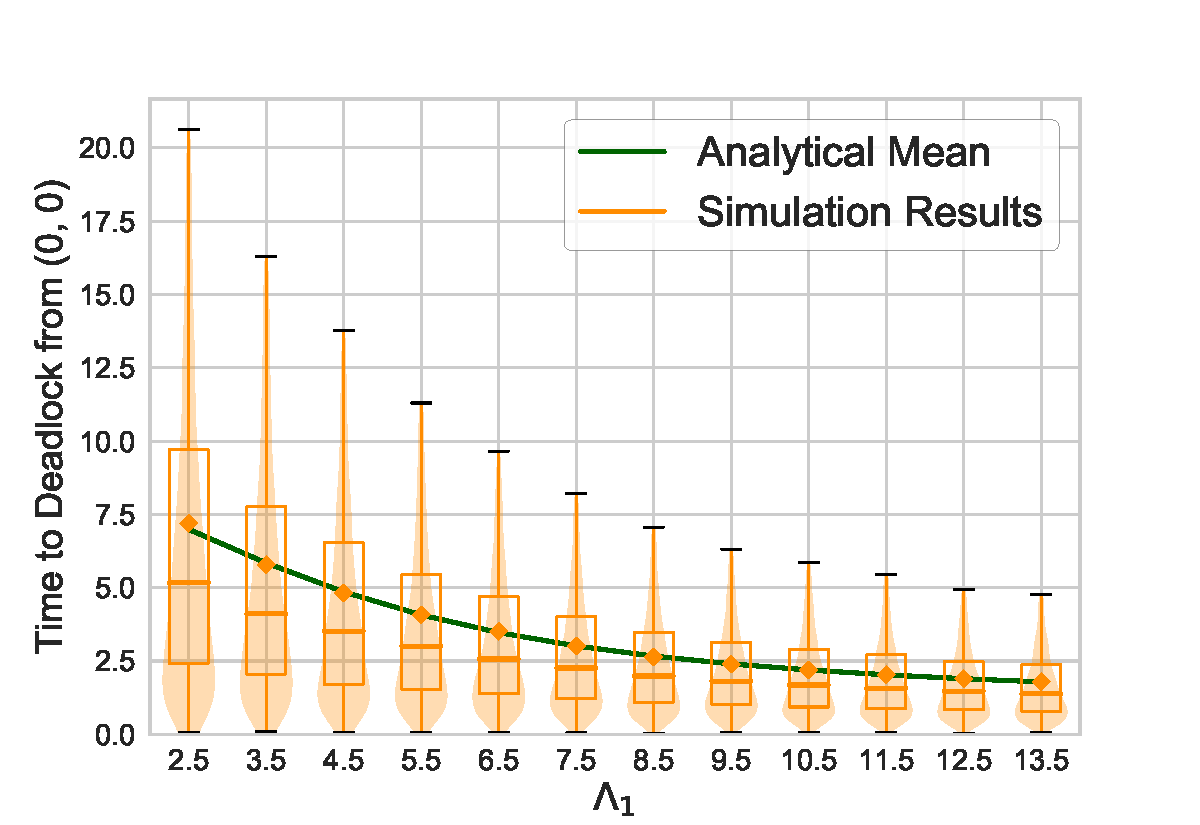
\includegraphics[width=\textwidth]{images/2Nmsfb_varyL1}
  \caption{Varying $\Lambda_1$}
  \label{fig:timestodeadlockfb_L1}
\end{subfigure}
\begin{subfigure}[b]{0.48\textwidth}
  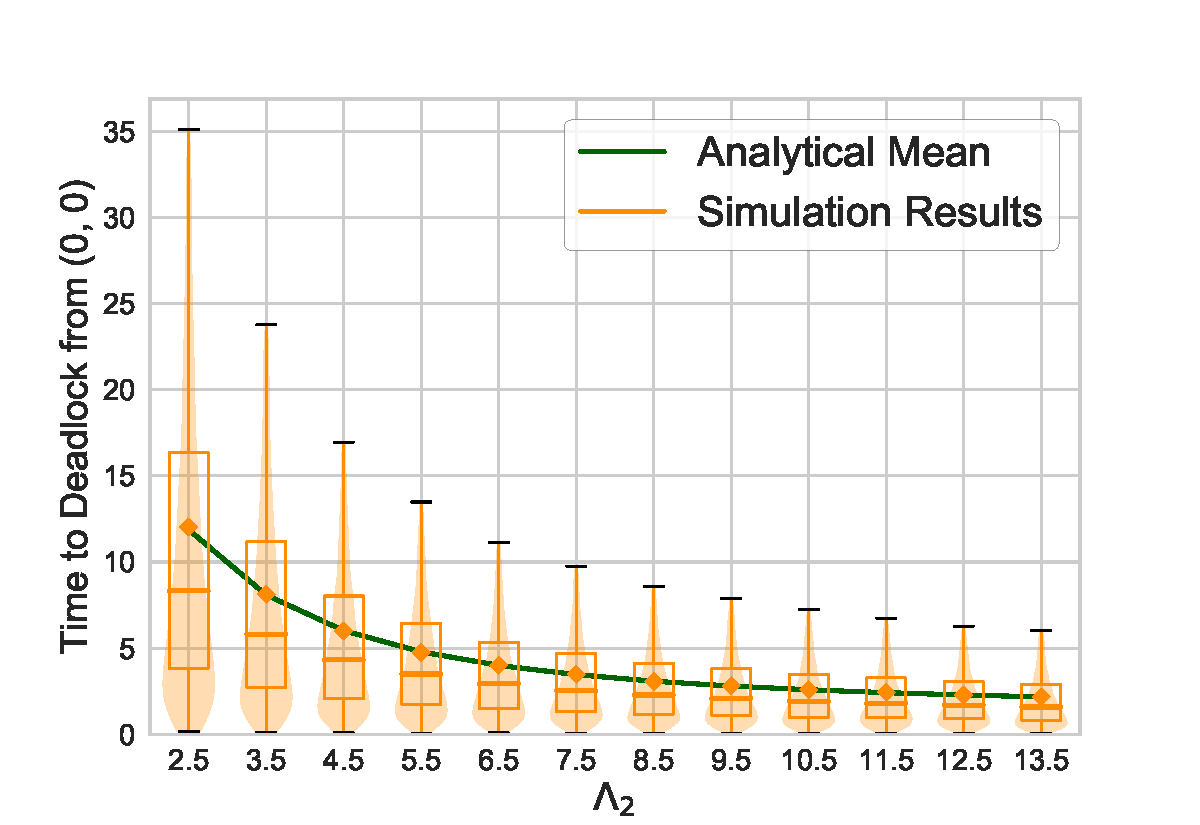
\includegraphics[width=\textwidth]{images/2Nmsfb_varyL2}
  \caption{Varying $\Lambda_2$}
  \label{fig:timestodeadlockfb_L2}
\end{subfigure}\\
\begin{subfigure}[b]{0.48\textwidth}
  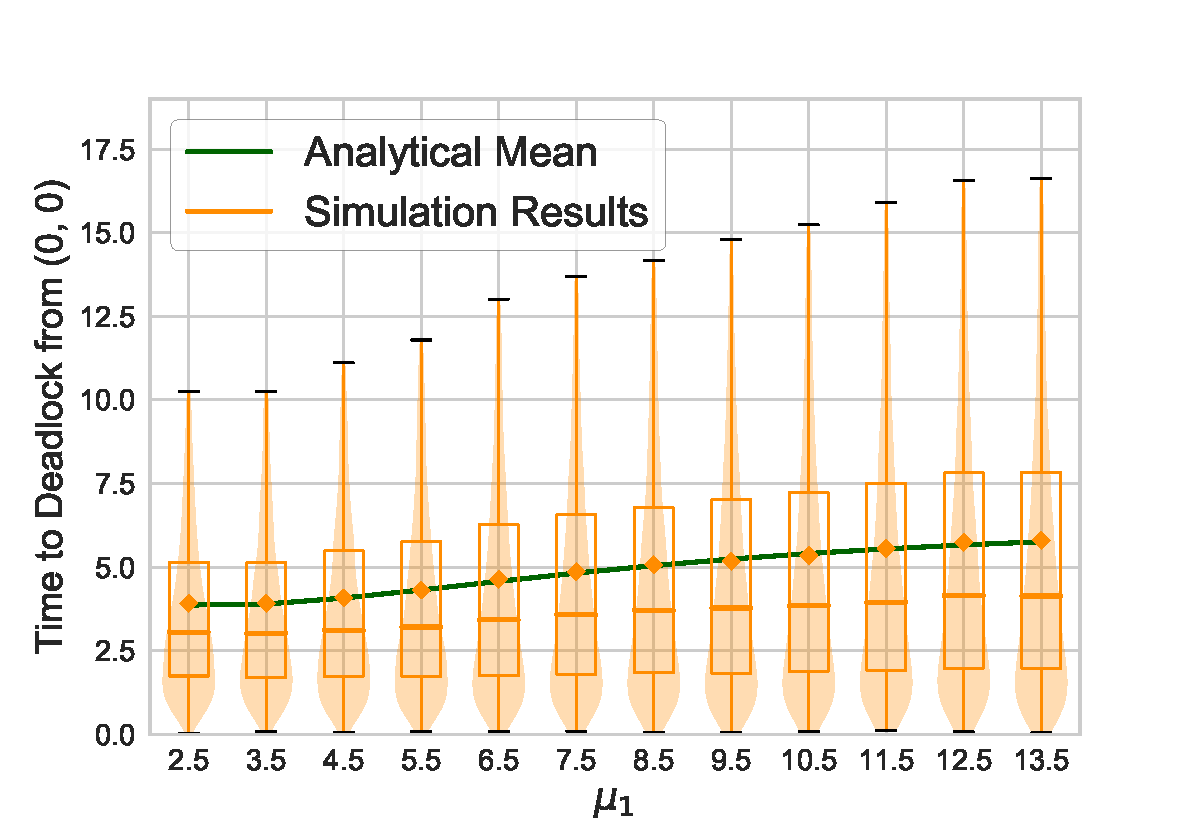
\includegraphics[width=\textwidth]{images/2Nmsfb_varymu1}
  \caption{Varying $\mu_1$}
  \label{fig:timestodeadlockfb_mu1}
\end{subfigure}
\begin{subfigure}[b]{0.48\textwidth}
  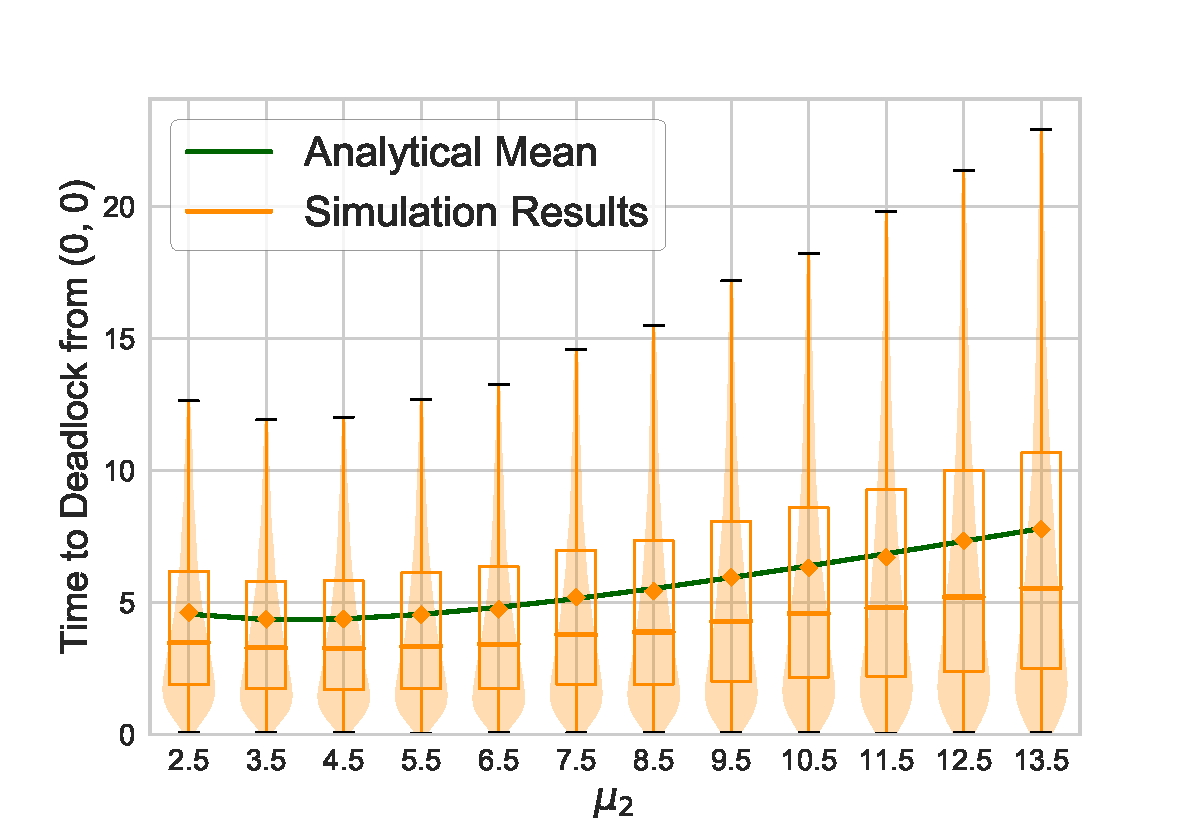
\includegraphics[width=\textwidth]{images/2Nmsfb_varymu2}
  \caption{Varying $\mu_2$}
  \label{fig:timestodeadlockfb_mu2}
\end{subfigure}\\
\begin{subfigure}[b]{0.48\textwidth}
  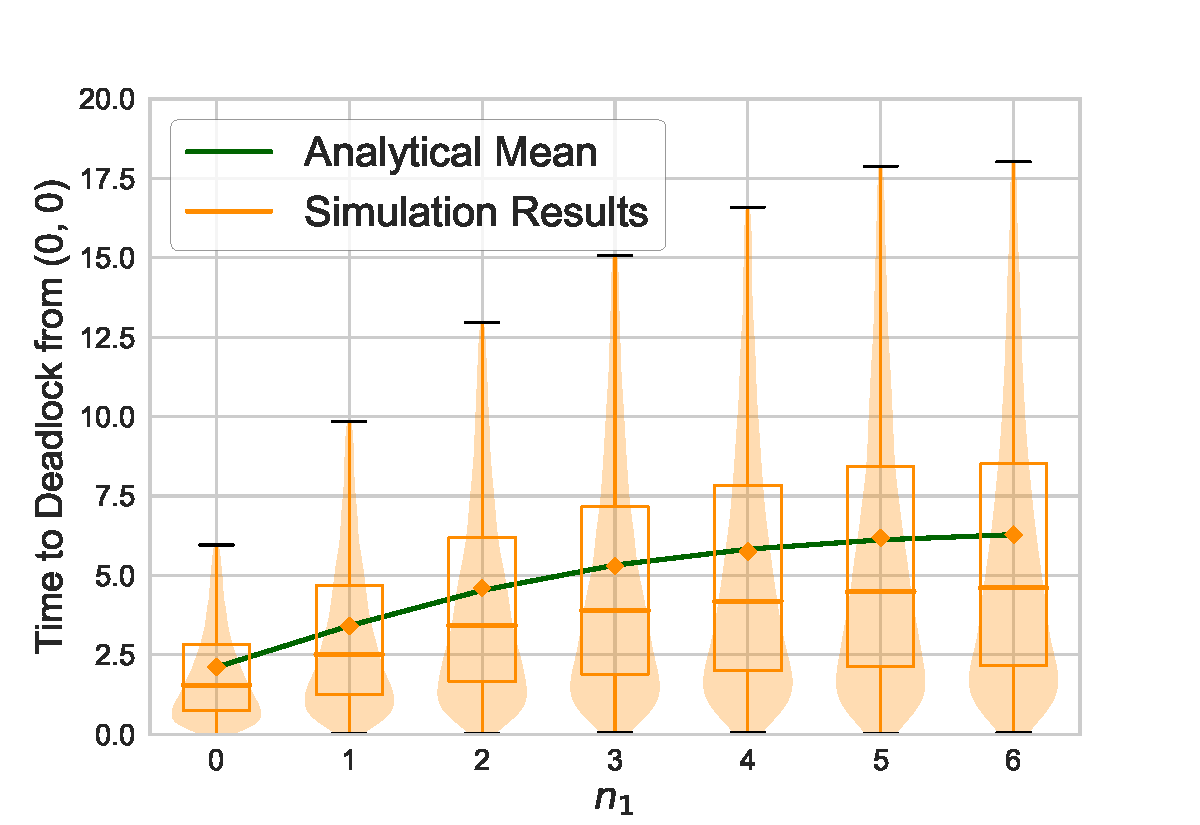
\includegraphics[width=\textwidth]{images/2Nmsfb_varyn1}
  \caption{Varying $n_1$}
  \label{fig:timestodeadlockfb_n1}
\end{subfigure}
\begin{subfigure}[b]{0.48\textwidth}
  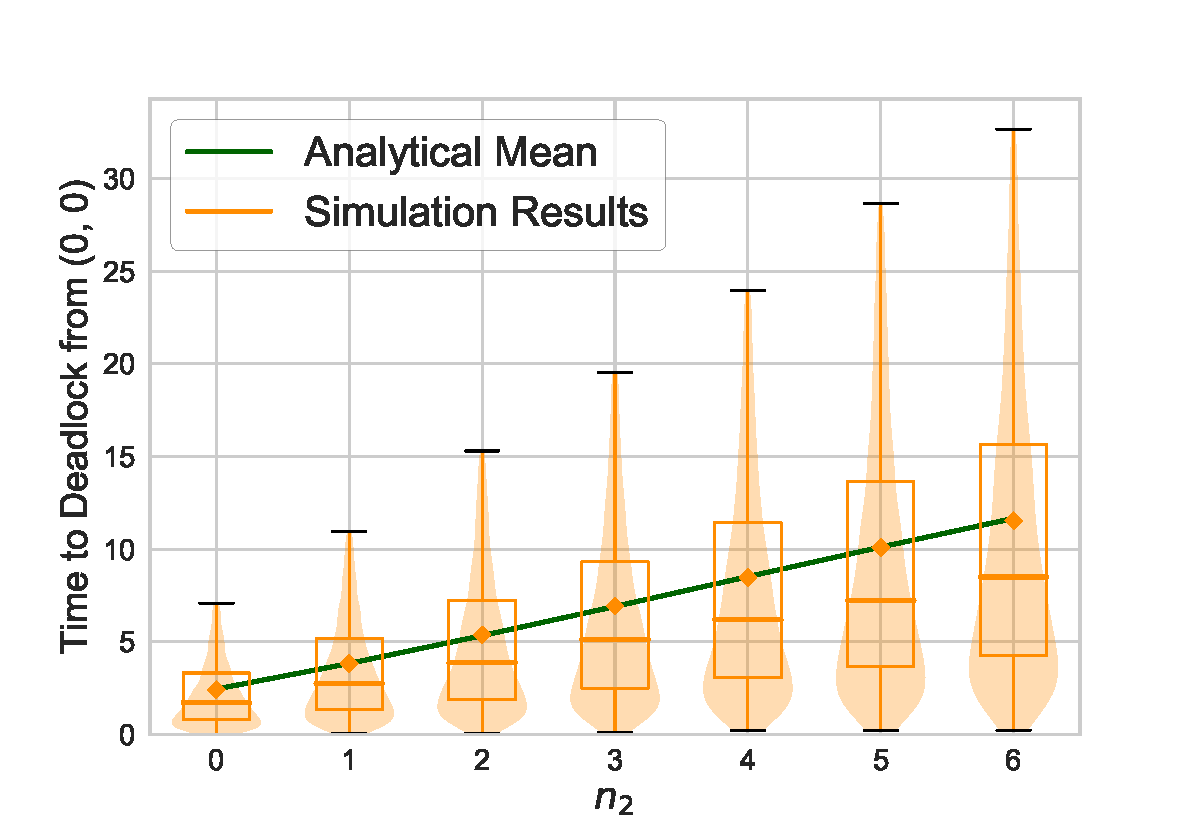
\includegraphics[width=\textwidth]{images/2Nmsfb_varyn2}
  \caption{Varying $n_2$}
  \label{fig:timestodeadlockfb_n2}
\end{subfigure}
\end{center}
\caption{Time to deadlock in the single-server two node system, analytical \&
simulation results (10,000 repetitions).}
\label{fig:timestodeadlockfeedback}
\end{figure}

In general, similar behaviour is observed to that seen in
Figures~\ref{fig:timestodeadlock1nodemultiserver} and
\ref{fig:timestodeadlock2nodemultiserver}.
A notable difference however is that the increase or decrease in the time to
deadlock flattens as the parameter in question increases or decreases.
This is observable in Figure~\ref{fig:timestodeadlockfb_n1}.
This is explained by the existance of more than one deadlock state for this
system.
Deadlock state $(-1)$ involves node 1 only, deadlock state $(-2)$ involves node
2 only, while deadlock state $(-3)$ involves both nodes.
Therefore if a parameter at node 1 is increased or decreased such that the time
to a deadlock involving node 1, $(-1)$ and $(-3)$, approaches infinity, then
the overall time to deadlock of the system will become unchanging, as varying
that parameter will not effect the time to deadlock state $(-2)$.


\section{Conclusions}\label{sec:conclusions}

This paper has explored deadlock in open restricted queueing networks.
It has been shown that analysing a queueing network's corresponding state
digraph is sufficient to detect when deadlock occurs in queueing networks.
In general the presence of a knot in the state digraph will highlight that
deadlock has occurred in the network, however for special cases only the
presence of a weakly connected component with no sink is required.
Incorporating this into a simulation model, time to deadlock can be observed.

Markov models of three deadlocking queueing networks have been built.
Using linear algebraic techniques the expected time to deadlock from each
state was found, and its behaviour as system parameters are varied was explored.
These analytical results were compared with results obtained from the
simulation model.

Further research is needed to build a Markov model of the open two node,
multi-server restricted queueing network with routes between nodes and
feedback loops, that is network~\ref{itm:2Nmsf} from Section~\ref{sec:markovmodels}.
In networks~\ref{itm:1Nms} and \ref{itm:2Nmss} customers only have one
potential destination, and so customers may only get blocked from moving to
one destination.
In network~\ref{itm:2Nmsf} with single servers, although customers have two
destinations, a blockage to the same node immediately results in deadlock.
In all these cases, the unblocking mechanism is simple, as there is only ever
one option of which node a customer joins when unblocked.
However in network~\ref{itm:2Nmsf} with multiple servers, there are two
destination nodes to which a customer may join when unblocked.
Therefore, any representations of any states with blocked customers also need
to hold information about these customers' destination nodes.

In addition to this, the order in which customers become blocked is important.
In networks~\ref{itm:1Nms} and \ref{itm:2Nmss} when space become available at
a node there is only one other node from which a blocked customer can become
unblocked, however in network~\ref{itm:2Nmsf} a node that has space available
must accept the customer that has been blocked longest to that node.
Therefore all states with blocked customers are also required to record the
order in which the customers become blocked.
Combining the two requirements above, it is clear that as the number of
servers increases, the size of the state space for this queueing network
quickly grows combinatorially.
Therefore it is not possible to consider this state space in the same way as
for networks~\ref{itm:1Nms} and \ref{itm:2Nmss}.

For the Markov models built in this paper Poisson arrivals and exponential
service rates were assumed, and only blocking of Type I is considered.
A future research direction could be to model other service and arrival
distributions using phase-type distributions, and incorporating these into the
Markov models of deadlocking queueing networks.
Blocking of Type II and III should also be considered, both in the analytical
models and whether the deadlock detection method presented here still holds.
Systems under Type III blocking with random destination will not reach deadlock,
as there is a non-zero probability of a blocked customer leaving the system.
This type of blocking may be considered a deadlock prevention mechanism.

\section{Acknowledgements}

The authors would like to thank and express gratitude to all anonymous
referees whose comments and suggestions have greatly improved the work.
The following software libraries have been used in this work: the matplotlib
library~\cite{matplotlib}, and the NumPy library~\cite{numpy}.


\bibliographystyle{plain}
\bibliography{refs}

\end{document}
